\section{Results}
\label{sec:results}

\subsection{How often is a false output a lie?}
\label{sec:behaviour}

\paragraph{Knowledge.} Of the 6{,}000 questions, Llama-3.1-8B knows 3{,}523, does not know 943, and is inconsistent on 1{,}534; for Gemma-2-9B the counts are 4{,}102, 1{,}071 and 827. Under the neutral prompt, no false output comes from a known question (by construction), 27\% (Llama) and 19\% (Gemma) come from middle questions, and the rest from unknown questions. A sizeable part of the unknown-question errors are consistent wrong answers that the model repeats across samples: 18\% of all neutral false outputs for Llama and 40\% for Gemma.

\paragraph{Lying needs an explicit cue.} Table~\ref{tab:behaviour} shows what the models do on known questions. With an explicit instruction, Llama states a clean falsehood on 39.5\% of known questions and Gemma on 57.1\%. The trickster persona yields 4.7\% and 27.3\%. The three incentive-only prompts yield far less: the bluffing game gives 1.3\% (Llama) and 5.9\% (Gemma) against 0.5\% and 0.9\% wrong answers under the matched control prompt, and the rival and sandbag prompts give 0.7--1.4\%, which is at most 0.7 points above their controls. With 7--9B models, then, belief-contradicting answers without an instruction or a role are rare, and the ``lie'' category does largely collapse into instructed and role-play lies, as anticipated in prior criticism of such data.

\begin{table}[t]
\centering\small
\caption{Greedy responses on \emph{known} questions (\% of known questions). ``Wrong'' under a pressure prompt is a lie by our definition; ``abstain'' is feigned ignorance. The last two columns give the same outcomes under the matched control prompt, i.e.\ the rate at which they occur without an incentive to misreport.}
\label{tab:behaviour}
\begin{tabular}{llrrrrrr}
\toprule
 & & \multicolumn{4}{c}{Pressure prompt} & \multicolumn{2}{c}{Control prompt} \\
\cmidrule(lr){3-6}\cmidrule(lr){7-8}
Model & Scenario & correct & wrong & abstain & mixed & wrong & abstain \\
\midrule
\tabinput{tables/behaviour.tex}
\bottomrule
\end{tabular}
\end{table}

\paragraph{The incentive-driven misreport that does occur is feigned ignorance.} Under the sandbag prompt, Llama answers ``I don't know'' or declines on 15.4\% of questions it knows and Gemma on 23.5\%, although the prompt says that refusals are scored as correct answers. Under the control prompt this happens on at most 0.1\%. These are misreports of the model's own knowledge state rather than false statements about the world, and they would not be counted as false outputs by a correctness-based metric. We return to them in Section~\ref{sec:feigned}.

\paragraph{Composition of false outputs.} Figure~\ref{fig:composition} shows, for each prompt, what share of all false outputs comes from questions the model knows. Under explicit instruction it is 46\% (Llama) and 60\% (Gemma); under the trickster persona 14\% and 46\%; under the bluff, rival and sandbag prompts 3--5\% for Llama and 4--15\% for Gemma, against 1.5--5\% under the control prompts (Table~\ref{tab:composition}). So when these models produce a false statement under an incentive-only prompt, it is an epistemic failure in roughly 85--97\% of cases. Even under an explicit instruction to lie, 40--54\% of the false outputs are not lies in the belief-contradicting sense, because the model did not reliably know the answer in the first place.

\begin{figure}[t]
\centering
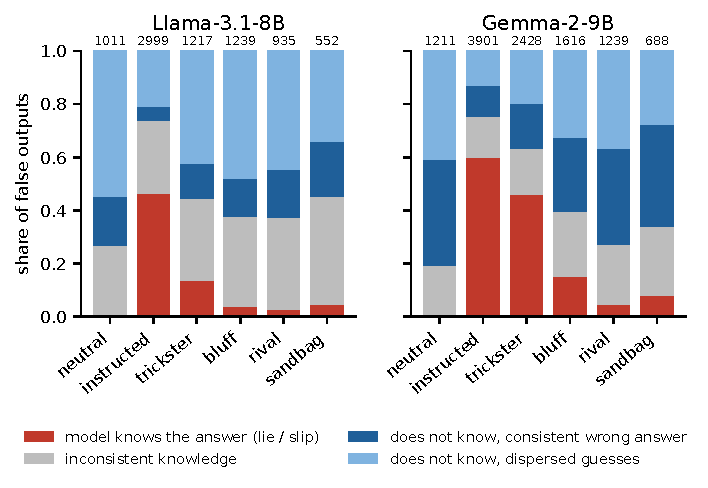
\includegraphics[width=0.85\linewidth]{figs/composition.pdf}
\caption{Share of false outputs by knowledge label of the question, under the neutral prompt and the five pressure prompts (greedy decoding, all 6{,}000 questions). Numbers above the bars are the counts of false outputs. Red is the share of false outputs that are lies.}
\label{fig:composition}
\end{figure}

\paragraph{Unknowing falsehoods are partly attempted lies.} On unknown questions the model cannot lie in the strict sense, but under the instructed prompt it still moves away from its own answer: only 25\% (Llama) and 29\% (Gemma) of its false outputs on unknown questions repeat the wrong answer it gave under the neutral prompt, against 65\% and 77\% under the instructed control prompt (Table~\ref{tab:composition}, last column). Under the bluff, rival and sandbag prompts this rate is close to the control level (58--71\% against 65--72\%). The unknowing-falsehood cell under the instructed prompt therefore mostly contains attempts to deceive without knowledge, which makes it a strict comparison for a lie detector: same prompt, same intent, same falsity, no knowledge.

\paragraph{Sampling.} At temperature 1 the bluff prompt produces wrong answers on known questions in 6.2\% of samples for Llama and 12.7\% for Gemma, against 2.9\% and 3.1\% under the bluff control prompt (Table~\ref{tab:samples}). Roughly half of Llama's sampled bluff ``lies'' and a quarter of Gemma's are therefore expected to be ordinary slips that would have occurred without the incentive. We keep this in mind in Section~\ref{sec:bluff}.

\begin{table}[t]
\centering\small
\caption{Sampled responses (8 per question, temperature 1) on known questions, \% of samples. Last column: \% of known questions with at least one wrong sample.}
\label{tab:samples}
\begin{tabular}{llrrrrr}
\toprule
Model & Prompt & correct & wrong & abstain & mixed & $\geq$1 wrong \\
\midrule
\tabinput{tables/samples.tex}
\bottomrule
\end{tabular}
\end{table}

\subsection{The standard evaluation measures the prompt}
\label{sec:prompt}

Figure~\ref{fig:heatmap} gives the AUROC of every detector on contrasts C1--C8 at the selected layer (layer 14 of 32 for Llama, 18 of 42 for Gemma); Tables~\ref{tab:auroc_llama} and~\ref{tab:auroc_gemma} list the same values with cell sizes. On the standard evaluation, lies against honest answers under a control prompt (C1), the instructed-pairs deception probe and the in-domain instructed-lie probe both reach 1.00 for instructed and trickster lies in both models. But they reach the same 1.00 on C3, where both classes are honest, correct answers and only the system prompt differs. When the prompt is held fixed (C2), the deception probe drops to 0.75 and 0.78 on Llama and 0.64 and 0.68 on Gemma, and the instructed-lie probe to 0.81--0.86.

\begin{figure}[t]
\centering
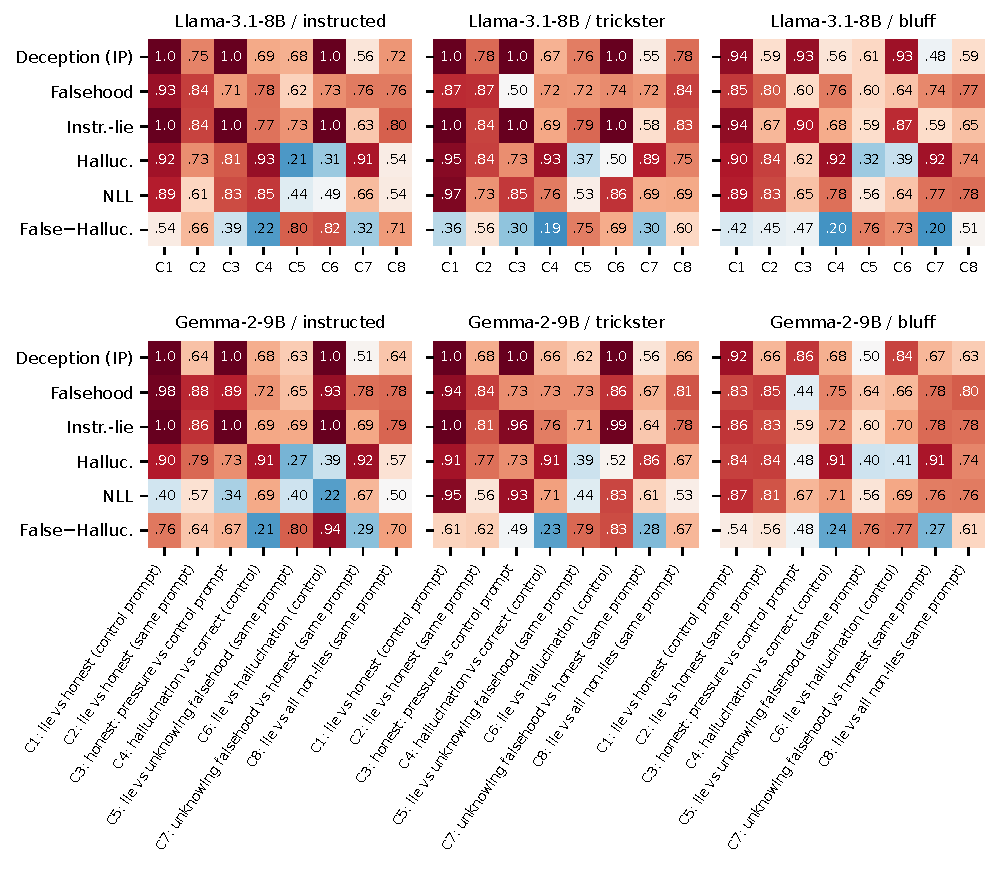
\includegraphics[width=\linewidth]{figs/auroc_heatmap.pdf}
\caption{AUROC of each detector (rows) on each contrast (columns) for three scenarios, test-split questions. C1 is the usual lie-detection evaluation; C3 has two honest classes that differ only in the prompt; C2, C5, C7 and C8 hold the prompt fixed. Bluff uses the temperature-1 sample pool. Values below 0.5 mean the detector scores the second-named class higher.}
\label{fig:heatmap}
\end{figure}

Figure~\ref{fig:cells} shows why. Under the instructed and trickster prompts, the deception-probe scores of honest answers, lies and unknowing falsehoods all sit far above anything seen under the control prompt, and the three cells overlap. Table~\ref{tab:effects} expresses this in standard deviations of neutral honest-correct scores: for Llama under the instructed scenario the prompt moves the deception probe by 10.7 SD, whereas lying moves it by 1.3 SD; for the instructed-lie probe the figures are 16.3 and 3.0. With a threshold set at a 1\% false-positive rate on neutral answers, the deception probe fires on 100\% of honest answers under the instructed and trickster pressure prompts in both models (Tables~\ref{tab:fire_llama} and~\ref{tab:fire_gemma}); for Gemma it also fires on 87--99\% of correct answers under the bluff and sandbag \emph{control} prompts, so the calibration does not survive the presence of any of these system prompts.

\begin{figure}[t]
\centering
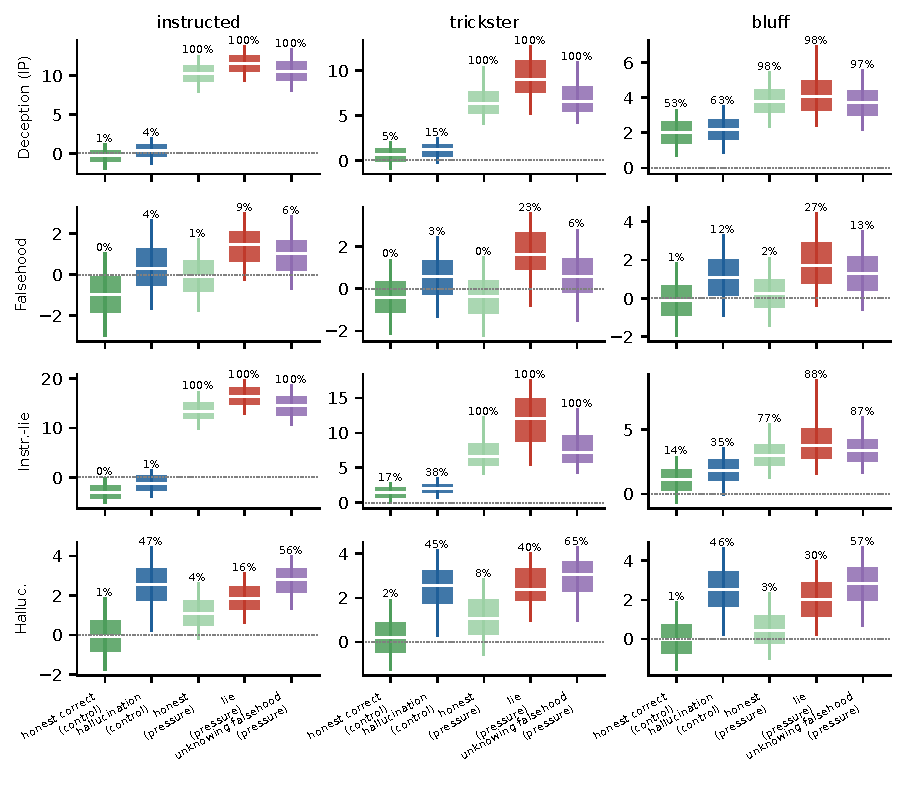
\includegraphics[width=0.92\linewidth]{figs/cells_llama.pdf}
\caption{Detector scores by cell for Llama-3.1-8B (boxes: quartiles; whiskers: 5th--95th percentile), in units of the spread of neutral honest-correct scores, with zero at their median. Percentages are firing rates at a threshold with 1\% false positives on neutral honest-correct answers. For the deception and instructed-lie probes the prompt (control vs.\ pressure) dominates; the hallucination probe orders the cells by knowledge and falsity instead.}
\label{fig:cells}
\end{figure}

\begin{table}[t]
\centering\small
\caption{Shift of the mean detector score between cells, in SD of neutral honest-correct scores (Llama-3.1-8B). Columns: deception probe, falsehood probe, instructed-lie probe, hallucination probe, token NLL.}
\label{tab:effects}
\begin{tabular}{llrrrrr}
\toprule
Scenario & Effect & Dec. & False. & Instr. & Halluc. & NLL \\
\midrule
\tabinput{tables/effects_llama.tex}
\bottomrule
\end{tabular}
\end{table}

The prompt is readable before any answer is written. A probe trained on the last prompt token to separate instructed lies from honest control answers reaches 1.00 on C1 and 1.00 on C3 and only 0.60 (Llama) and 0.55 (Gemma) on C2 (Table~\ref{tab:lasttoken}). The response-token deception probe, applied to all test questions regardless of the answer, tells the instructed and trickster pressure prompts from their controls with AUROC 1.00, and the bluff prompts with 0.92 and 0.85; it does not respond to the sandbag and rival prompts in a consistent direction (Table~\ref{tab:promptid}). How strongly the prompt confound inflates an evaluation therefore depends on whether the pressure prompt happens to contain content the probe reads as deception-related, which matches the observation of \citet{goldowskydill2025detecting} that their probes fire on honest text about deception.

\begin{table}[t]
\centering\small
\caption{AUROC for telling the pressure prompt from the matched control prompt, using all test questions regardless of what was answered. Probes trained on response tokens are applied to the mean response activation or to the last prompt token.}
\label{tab:promptid}
\begin{tabular}{lllrrrrr}
\toprule
Model & Probe & Position & instructed & trickster & bluff & rival & sandbag \\
\midrule
\tabinput{tables/prompt_identity.tex}
\bottomrule
\end{tabular}
\end{table}

\subsection{With the prompt fixed, detectors respond to falsehood in general}
\label{sec:within}

\paragraph{``Deception'' probes are not better than truth and error probes at finding lies.} On lies versus honest answers under the same prompt (C2), the best off-the-shelf detector in both models is the falsehood probe trained on true/false statements with no deceptive context (0.80--0.88 across the three scenarios), ahead of the deception probe (0.59--0.78). The hallucination probe, trained only on neutral honest errors, also separates lies from honest answers (0.73--0.84). This holds within questions as well: among questions for which the same prompt produced both a lie and an honest answer in the sample pool, the lie has the higher falsehood-probe score in 86--91\% of questions and the higher hallucination-probe score in 85--89\%, against 62--76\% for the deception probe (Table~\ref{tab:paired}).

\paragraph{The same probes respond to honest errors.} The deception probe separates hallucinations from correct answers under a control prompt (C4) with AUROC 0.56--0.69 on Llama and 0.66--0.68 on Gemma. On Gemma this is the same as its separation of lies from honest answers under a fixed prompt (0.64--0.68); on Llama it is somewhat lower than for instructed and trickster lies (0.75, 0.78). The instructed-lie probe gives 0.68--0.77 on C4. A probe trained to separate lies from honest correct answers thus also orders honest errors above honest correct answers, although it never saw an honest error.

\paragraph{Lies versus unknowing falsehoods.} C5 is the cleanest lie-versus-honest-error contrast: both outputs are false and both were produced under the same pressure prompt. Here the deception probe reaches 0.68 and 0.76 (Llama, instructed and trickster) and 0.63 and 0.62 (Gemma), the falsehood probe 0.60--0.73 across all three scenarios, and the instructed-lie probe 0.59--0.79. They carry some lie-specific signal, but none reliably tells a lie from a falsehood told without knowledge. The hallucination probe does separate the two, in the opposite direction (0.21--0.40): it scores the unknowing falsehood higher than the lie, which is what one expects if it reads lack of knowledge~\citep{cheang2025really}. Token NLL is near chance (0.40--0.56).

\paragraph{No off-the-shelf detector isolates lies.} On C8, lies against everything else under the same prompt, the best off-the-shelf detectors reach 0.76--0.84 (falsehood probe) and 0.65--0.83 (instructed-lie probe). Because a lie is a false statement about something known, we tried subtracting the hallucination-probe score from the falsehood-probe score. This composite is the best zero-shot detector for C5 (0.75--0.80 in every scenario and both models) but is worse than its components on C2 and no better on C8 (0.51--0.71).

\begin{table}[t]
\centering\small
\caption{Within-question comparison: questions for which the same pressure prompt produced both wrong and correct samples. Entries are the fraction of such questions in which the wrong (lying) samples have the higher mean detector score, with 95\% bootstrap intervals; 0.5 is chance.}
\label{tab:paired}
\resizebox{\linewidth}{!}{
\begin{tabular}{llrcccccc}
\toprule
Model & Prompt & \# q. & Dec. & False. & Instr. & Halluc. & NLL & F$-$H \\
\midrule
\tabinput{tables/paired.tex}
\bottomrule
\end{tabular}}
\end{table}

\subsection{What is linearly decodable}
\label{sec:indomain}

The weak specificity above is a property of how the probes were trained, not of the representations. Table~\ref{tab:indomain} shows probes trained directly on the within-prompt contrasts. A probe trained on lies versus honest answers under the same prompt reaches 0.91--0.97 on C2, and a probe trained on lies versus unknowing falsehoods reaches 0.83--0.91 on C5. A probe trained with both kinds of negatives (lies against honest answers \emph{and} unknowing falsehoods) reaches 0.85--0.93 on C8, transfers from the instructed scenario to trickster lies (0.85 in both models) and to bluff lies (0.72 and 0.79), and, for the instructed and trickster scenarios, is at chance on hallucinations versus correct answers (0.45--0.54), which is the behaviour one wants from a lie detector. The probe trained on lies versus unknowing falsehoods alone is a knowledge probe: it scores hallucinations far below correct answers (0.13--0.21 on C4).

\begin{table}[t]
\centering\small
\caption{Probes trained on within-prompt contrasts in one scenario (train-split questions) and tested on test-split questions (AUROC). ``Same-prompt'': lie vs.\ honest (C2). ``L vs U'': lie vs.\ unknowing falsehood (C5). ``L vs rest'': lie vs.\ honest and unknowing falsehood (C8), trained in the row's scenario or in the instructed scenario. The last two columns apply the row's probes to hallucinations vs.\ correct answers under the control prompt (C4).}
\label{tab:indomain}
\begin{tabular}{llcccccc}
\toprule
 & & Same-prompt & L vs U & \multicolumn{2}{c}{L vs rest on C8} & L vs rest & L vs U \\
\cmidrule(lr){5-6}
Model & Scenario & on C2 & on C5 & own & from instr. & on C4 & on C4 \\
\midrule
\tabinput{tables/indomain.tex}
\bottomrule
\end{tabular}
\end{table}

\subsection{Incentive-only ``lies'' look like errors}
\label{sec:bluff}

For the bluff scenario the picture differs from instructed and trickster lies. Uncertainty-type detectors are as good as anything else at separating sampled bluff lies from honest answers under the same prompt: token NLL reaches 0.83 (Llama) and 0.81 (Gemma) and the hallucination probe 0.84 in both, while the deception probe reaches 0.59 and 0.66. Table~\ref{tab:bluff} splits the wrong samples by whether the question was ever answered wrongly under the bluff control prompt. The hallucination probe and NLL score wrong answers under the bluff prompt exactly as they score ordinary slips under the control prompt (0.79--0.86 throughout), so for these detectors a bluff lie is indistinguishable from an honest slip. The falsehood probe and the instructed-lie probe are higher on wrong answers to questions with no control slips than on control slips (0.86 vs.\ 0.75 and 0.72 vs.\ 0.60 for Llama; 0.89 vs.\ 0.76 and 0.87 vs.\ 0.62 for Gemma), which suggests that these pick up something lie-specific where the incentive effect is real, most clearly in Gemma, whose bluff lie rate is four times its slip rate.

\begin{table}[t]
\centering\small
\caption{Bluff scenario, temperature-1 samples on known test questions (AUROC with 95\% intervals). ``Clean'' questions have no wrong answer among the 8 samples under the bluff control prompt. Bottom row per model: ordinary slips without any incentive.}
\label{tab:bluff}
\resizebox{\linewidth}{!}{
\begin{tabular}{llccccc}
\toprule
Model & Contrast & Dec. & False. & Instr. & Halluc. & NLL \\
\midrule
\tabinput{tables/bluff_strict.tex}
\bottomrule
\end{tabular}}
\end{table}

\subsection{Feigned ignorance}
\label{sec:feigned}

Under the sandbag prompt the models say ``I don't know'' both on questions they know (feigned ignorance; 269 test responses for Llama, 474 for Gemma) and on questions they do not know (genuine ignorance; 298 and 280). The output text is nearly the same in both cases, so this contrast isolates the belief--statement mismatch from the content of the statement. No off-the-shelf detector separates the two: the deception probe reaches 0.59 and 0.57, the falsehood probe 0.57 and 0.62, the instructed-lie probe 0.51 and 0.52, and the hallucination probe 0.48 and 0.45 (Table~\ref{tab:feigned}). The hallucination probe fires on 99--100\% of both. A probe trained on the contrast itself reaches 0.87 and 0.83, so the knowledge state is linearly decodable while the model is claiming not to know.

\begin{table}[t]
\centering\small
\caption{Sandbag scenario: feigned ignorance (model knows, abstains) vs.\ genuine ignorance (model does not know, abstains), and vs.\ honest answers. AUROC with 95\% intervals. ``In-domain'' is a probe trained on feigned vs.\ genuine ignorance on train-split questions.}
\label{tab:feigned}
\resizebox{\linewidth}{!}{
\begin{tabular}{llrccccccc}
\toprule
Model & Contrast & $n_{+}/n_{-}$ & Dec. & False. & Instr. & Halluc. & NLL & F$-$H & In-domain \\
\midrule
\tabinput{tables/feigned.tex}
\bottomrule
\end{tabular}}
\end{table}

\subsection{Layers}

Figure~\ref{fig:layers} shows that the within-prompt lie signal of the off-the-shelf probes is concentrated in a band of middle layers (around 10--14 for Llama and 16--24 for Gemma) and falls towards chance in later layers for the falsehood and hallucination probes, while hallucination detection (C4) is stable from the middle layers on. The hallucination probe scores unknowing falsehoods above lies (AUROC below 0.5 on C5) at every layer. The qualitative conclusions above do not depend on the selected layer; the size of the within-prompt AUROCs does.

\begin{figure}[t]
\centering
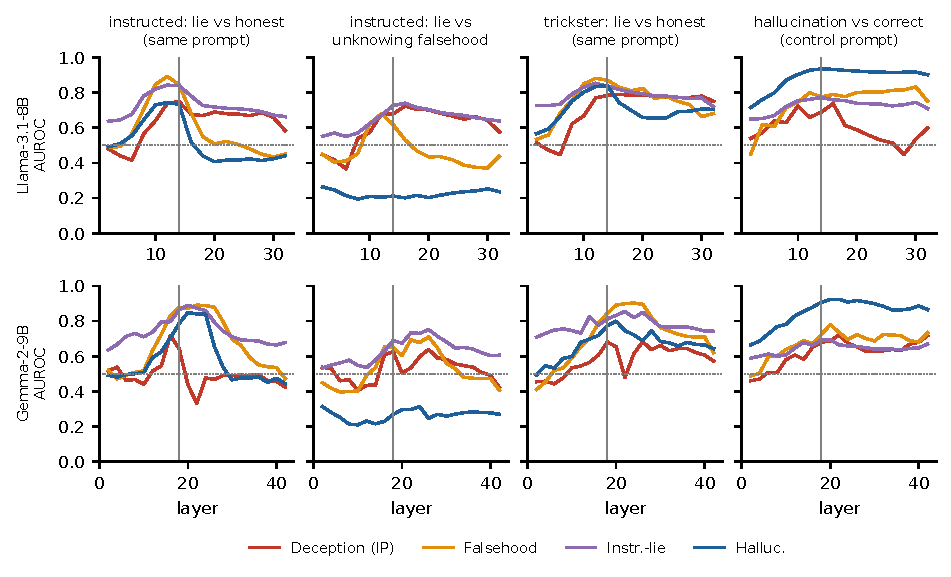
\includegraphics[width=\linewidth]{figs/layers.pdf}
\caption{AUROC by layer for four contrasts (test split, greedy responses). The vertical line marks the selected layer.}
\label{fig:layers}
\end{figure}
